\section{Graph Composer}
A graph is a mathematical object consisting of a set of vertices and edges that connect them, you may know a graph under the name network. Each vertex can have several attributes or values depending on what is being modeled. The edges can have direction, in which case we talk about a directed graph.

Graph Composer offers the possibility to compose music by walking along paths on a graph. In Graph Composer, each vertex is associated with a note and its duration over time. The edges connecting the vertices define a path along which one travels over time, meaning notes are played along the sequence of visited vertices. The sound obtained at each vertex takes on different shapes based on the decorator of the vertex, such as a pure note, a chord or arpeggio.

For example, the following score:
\begin{figure}[h]
\centering
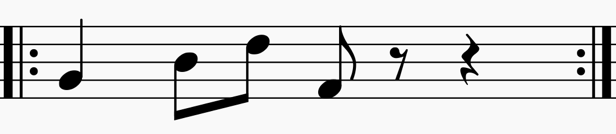
\includegraphics[width=0.5\textwidth]{GraphComposer_1}
\end{figure}

can be drawn as the following directed graph:
\begin{figure}[h]
\centering
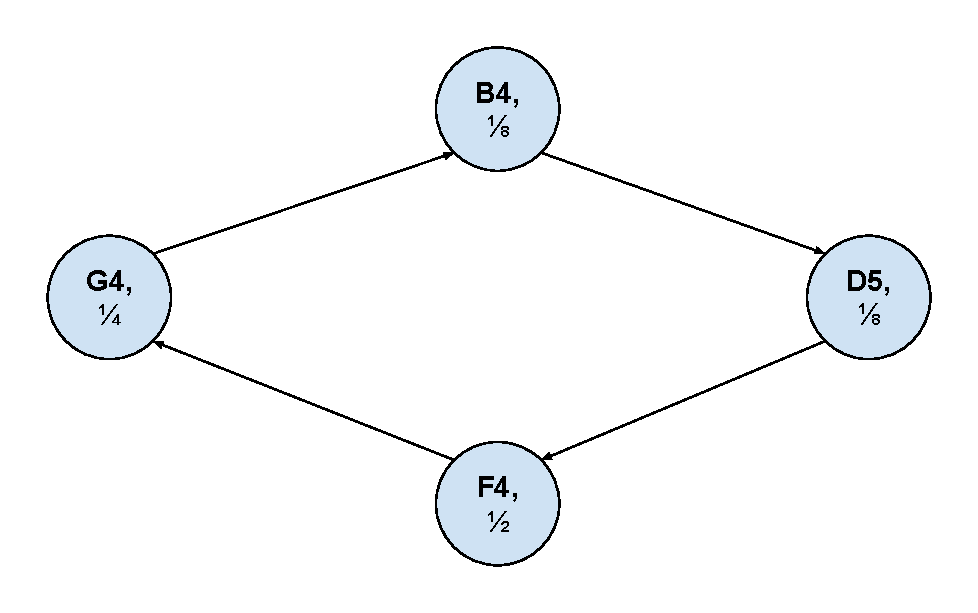
\includegraphics[width=0.5\textwidth]{GraphComposer_2}
\end{figure}

Paths on the graph represent sequences of notes. If the path has a loop, as in the example above, there is a repetition of a fragment. In the example, the graph has a unique possible path, but when there is more than one edge leaving a vertex, multiple paths are possible. 

For example, the following graph has two possible paths:

\begin{figure}[h]
\centering
\begin{subfigure}{0.45\textwidth}
\centering
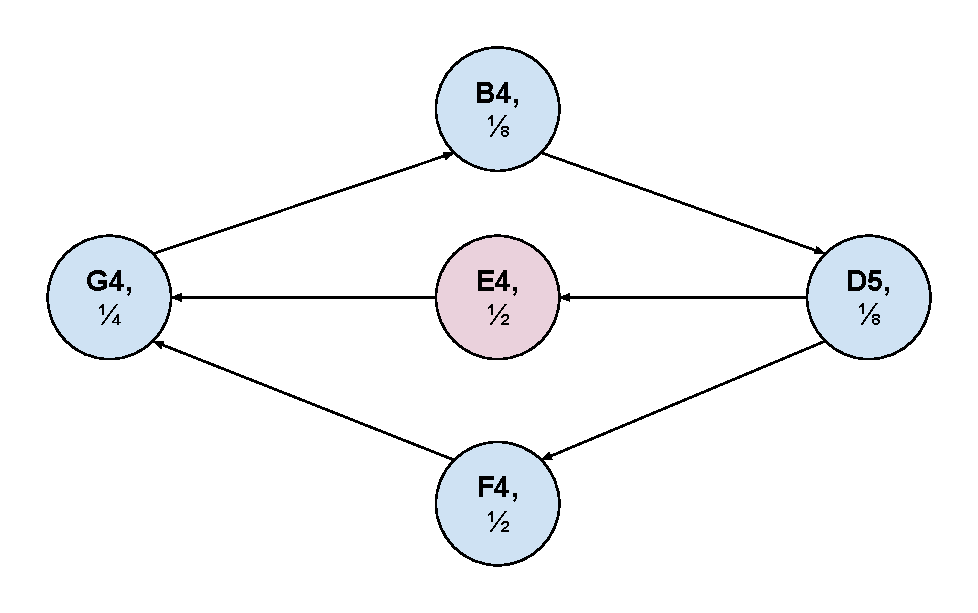
\includegraphics[height=3cm]{GraphComposer_3}
%\subcaption*{This graph can be walked through two paths.}
\end{subfigure}

\begin{subfigure}{0.45\textwidth}
\centering
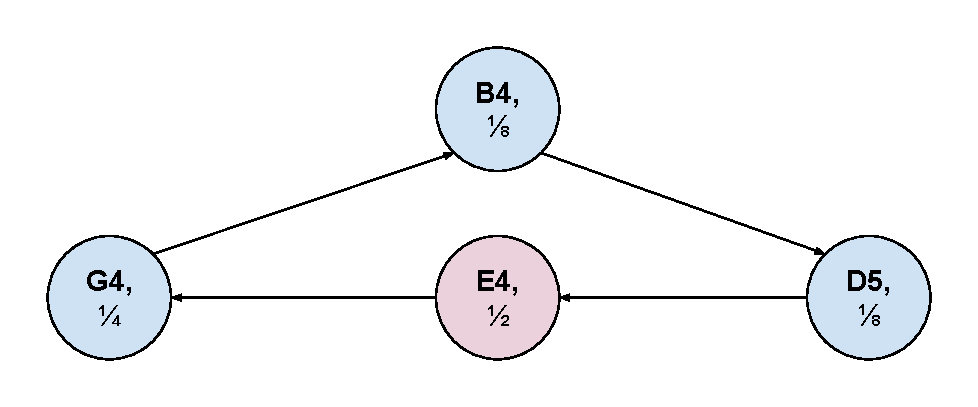
\includegraphics[width=\textwidth]{GraphComposer_5}
%\subcaption*{First path.}
\end{subfigure}
\begin{subfigure}{0.45\textwidth}
\centering
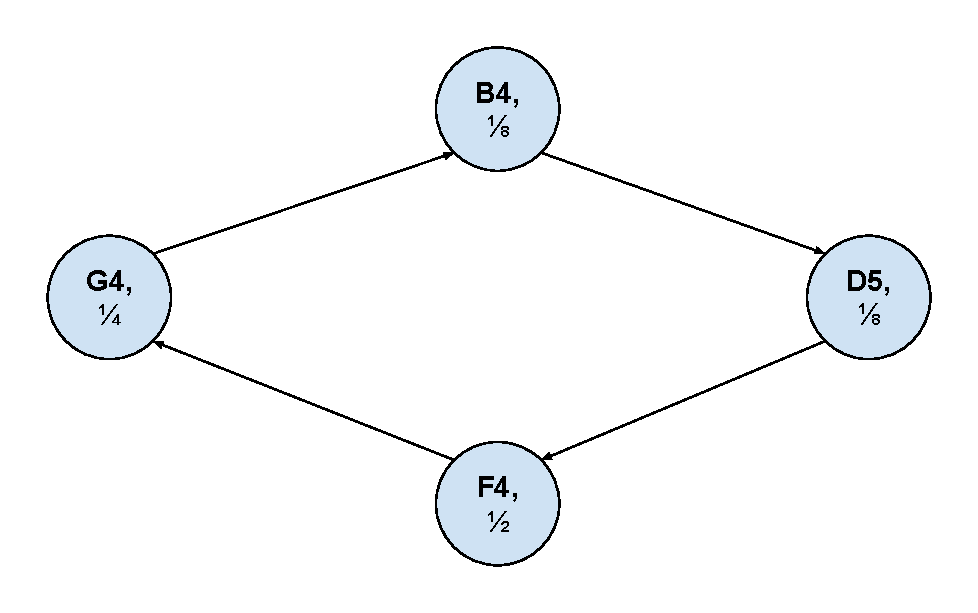
\includegraphics[width=\textwidth]{GraphComposer_4}
%\subcaption*{Second path.}
\end{subfigure}
\end{figure}

In this case, the program needs to make a choice in which way to follow the paths in the graph. Graph Composer chooses randomly between the two options (with equal probability), which creates what is called random walks through the graph. Since the music produced by each path may result in different lengths and therefor has a different overall duration for the music played, the listener will perceive this as some kind of ``un-rhythm''.

The model used by Graph Composer is used in Computational Musicology, a field of study where mathematics and computer science are applied to music. In research, musical compositions are modeled as graphs to compare and extract different mathematical features; for example, the number of times that a transition from one note to another is repeated, or the number of times that three (or more) different notes appear in the same sequence, amongst others.

Graph Composer walks paths randomly along the graph from the root vertex through the directed edges until it finds a vertex with no outward edges; then it returns to the root vertex. When the program is started, you can only see the root vertex (the only one that plays with no incoming edges). You can drag and add more vertices, change their notes, duration, and decoration. All of this can be done without the need to stop the music from playing. The complexity of the graph by adding many vertices and edges can quickly increase. Can you create patterns in your graph that create pleasant musical motifs? Happy listening.

\vfill

Authors of this exhibit: Pedro Arthur, Vitor Guerra Rolla, and José Ezequiel Soto Sánchez (Instituto de Matemática Pura e Aplicada, Brazil). 
Text: by the authors.

